\documentclass{acm_proc_article-sp}
\usepackage{graphicx}
\usepackage[plain]{fancyref}
\usepackage{listings}
\usepackage{color}
\definecolor{lightgray}{rgb}{.9,.9,.9}
\definecolor{darkgray}{rgb}{.4,.4,.4}
\definecolor{purple}{rgb}{0.65, 0.12, 0.82}
\DeclareMathOperator{\shapeOf}{shapeOf}

\lstdefinelanguage{JavaScript}{
  keywords={typeof, new, true, false, catch, function, return, null, catch, switch, var, if, in, while, do, else, case, break},
  keywordstyle=\color{blue}\bfseries,
  ndkeywords={class, export, boolean, throw, implements, import, this},
  ndkeywordstyle=\color{darkgray}\bfseries,
  identifierstyle=\color{black},
  sensitive=false,
  comment=[l]{//},
  morecomment=[s]{/*}{*/},
  commentstyle=\color{purple}\ttfamily,
  stringstyle=\color{red}\ttfamily,
  morestring=[b]',
  morestring=[b]"
}

\lstset{
   language=JavaScript,
   extendedchars=true,
   basicstyle=\small\ttfamily,
   showstringspaces=false,
   showspaces=false,
   numbers=left,
   numberstyle=\small,
   numbersep=9pt,
   tabsize=2,
   breaklines=true,
   showtabs=false,
   captionpos=b
}


\begin{document}

\title{A Reasonably Fast and Fully Capable JVM in JavaScript}

\numberofauthors{4}
\author{
\alignauthor Michael Bebenita
\alignauthor Brendan Dahl
\and
\alignauthor Marco Castelluccio
\alignauthor Myk Melez
\and
\alignauthor Andreas Gal
}

\maketitle
\begin{abstract}
Dramatic improvements in browser performance have now made JavaScript a viable compilation target for a wide range of programming languages.
While targetting JavaScript is fairly easy, navigating optimization tiers wrapped in arcane magic and mystery make squeezing performance out of modern JavaScript engines incredibly difficult.
In this paper we explore the implementation of a fully capable Java virtual machine in JavaScript.
One that supports: class loading, interpretation, dynamic compilation, on-stack-replacement, deoptimization, threading, synchronization, garbage collection, finalization, many of the other features that make Java, Java.
\end{abstract}

% \category{D.3.4}{Programming Languages}{Processors}

\terms{Languages, Design}

\keywords{ACM proceedings, \LaTeX, text tagging}

\section{Introduction}

Like it or not, JavaScript is the de facto lingua franca. ...
Lots of attempts at compiling to the web, C/C++ via Emscripten has be highly successful.
Java attempts have not been as successful, too slow, large code size.
Java needs class loading, it needs faster startup, low 
We believe compiling Java to JavaScript should be faster than writing JavaScript by hand.

The web pptimize for size and startup, not throughput.

\section{System Constraints}

In JavaScript you can't do this and that. No threads, no weak references, you can't do synch I/O, etc. ...
In JavaScript you have to pay for your cake before you eat it, vm code size matters.

\section{Motivation}



\section{Implementation}

\subsection{Class Loading}

Before the JVM can execute any code it must first load it.
Java classes are packaged in \texttt{.class} files and stored compressed in archive \texttt{.jar} files.
Decompressing \texttt{.jar} files is the first step in building a JVM in JavaScript and the first sign of the troubles ahead.

\subsubsection{GZip}

Archive files typically use the \texttt{DEFLATE} algorithm.
There are many JavaScript implementations of this algorithm, but none that we've been satisfied with in terms of performance.
...

\subsubsection{Class File Representation}

The most obvious way to deal with Java \texttt{.class} files is to parse them into a JavaScript friendly object graph.
This is convenient but it has several severe disadvantages:
\begin{enumerate}
\item The \texttt{.class} file structure is directly accessible and doesn't need to be parsed ahead-of-time.
Parsing introduces a significant latency delay and should be deferred as long much as possible. 
\item The \texttt{.class} file structure is compact. Reflecting this into an JavaScript object graph more than doubles the size of the data structure.
\end{enumerate}

To work around these limitations and still provide a convenient way to represent \texttt{.class} files, we create views on the underlying \texttt{.class} file buffer.
Access to most properties is performed via accessor getters that lazily construct additionaly subviews as needed.
The advantage of this approach is that most of the data is kept in the original buffer and never reflected into JavaScript properties.

\begin{figure}[htbp]
\begin{center}
\includegraphics[width=200px]{classInfo.pdf}
\caption{ClassInfo TypedArray Views}
\label{default}
\end{center}
\end{figure}

\subsubsection{Strings}

While it is tempting to reflect Java strings as JavaScript strings, it turns out that it is a lot more effective to keep them in their original representation.
Strings in modern JavaScript engines are heavily optimized.
Taking advantage of this fact seems like a good idea at first, not only for convenience but also for performance reasons.
Unfortunately reflecting Java strings as JavaScript strings causes a lot of unintended consequences:

\begin{enumerate}
\item Java \texttt{.class} files use a slightly modified UTF-8 string encoding scheme.
Decoding this scheeme is inefficient because JavaScript provides no efficient means of constructing strings from UTF-8 sequences.
More importantly, it is often unnecessary.
Most of the strings that appear in \texttt{.class} files are used for linking where comparisons and hashing are by far the most frequent operations.
Both of these operations are faster to implement on the original string representation and don't require UTF-8 decoding.
\item Java \texttt{.class} files contain a large number of strings, storing them in two different formats can take up a significant amount of memory.
\item Java's \texttt{String} class manages an internal \texttt{char []} array of characters.
This encoding is different from the encoding in the \texttt{.class} file but it would still need an associated JavaScript string to be kept in sync with the underlying char buffer.
\item Holding on to references to JavaScript objects from Java objects constrains the design of the Java object layout, as later described in \fref{sec:objectLayout}.
\end{enumerate}

\subsection{Object Layout} \label{sec:objectLayout}

The design of the object model has far reaching consequences.

\subsubsection{JavaScript Objects}
The straightforward approach is to model Java's inheritance hierarchy on top of JavaScript's prototypical inheritance chain (\fref{fig:objects} ()).
In this approach, each Java class is modeled as a JavaScript constructor \footnote{Java constructors are invoked explicity during bytecode execution and should no be confused with the JavaScript constructors in this case, the latter act more like object initializers.} function that initializes all of its fields to default values.
The function's default prototype object is linked up to the base class's default prototype and then populated with virtual methods.
JavaScript's prototype lookup mechanism takes care of the rest, emulating both virtual dispatch and interface dispatch.
% \footnote{Java classes may have duplicate field and/or method names, therefore signature should be used as unique identifiers.}

\begin{lstlisting}[caption=Simple Object Model]
function Object() {}
function Animal() {
	this.sibling = null;
}
Animal.prototype = 
	Object.create(Object.prototype); 
Animal.prototype.move = 
	function Animal_move () { };
function Snake() {
	this.sibling = null;
	this.length = 0;
}
Snake.prototype = 
	Object.create(Animal.prototype);
Snake.prototype.move = 
	function Snake_move () { };
Snake.prototype.bite = 
	function Snake_bite () { };

var snake = new Snake();
snake.length = 3;
snake.bite();
\end{lstlisting}

The main benefit of this approach is that it is easy to implement and understand.
It uses a every common code pattern that modern JavaScript VMs are highly tuned for.
These JavaScript objects have a highly regular structure, exactly the kind of structure that hidden class optimizations in JavaScript VMs are desinged to detect.

\paragraph{Field Access and Hidden Classes}
Conceptyally, all JavaScript objects are chained key/value ordered dictionaries.
Keys are usually strings \footnote{Even arrays for behave this way, keys are strings and don't necessarily need to be consecutive.} but values can vary in type.
All JavaScript objects have a hidden \texttt{\_\_proto\_\_} property that points to their prototype object.
If a property lookup fails on an object, the property search continues recursively along the prototype chain.
Cycles are not allowed in the prototype chain.
The model is simple, flexible and very powerful but it is very difficult to implement efficiently.
The most basic implementation of JavaScript objects uses chained hashtables.
All modern JavaScript VMs use hidden classes to detect the structure of objects and optimize property access.
The idea is farily simple.
As properties are added or removed from an object, the shape of the object changes.
The shape of the object identifies its internal structure and layout in memory.
The order in which properties are added to objects is important, so $\shapeOf(\{x: 1, y: 2\}) \neq \shapeOf(\{y: 2, x: 1\})$, 
however $\shapeOf(\{x: 1, y: 2, z: 3\}) \subset \shapeOf(\{x: 1, y: 2\})$ since it shares part of the shape.
The shape of an object also depends on the shape of its prototype, mutations along the prototype chain can potentially modify the shape of many objects.

At a property access site, if the previously observed shape of the receiver object still holds, then the compiled code can take a faster code path where the property directly accessed at a known slot offset.
If the object's shape has changed, the VM bails out of compiled code and resumes execution in an interpreter or baseline-compiler.
These types of speculative optimizations are the bread and butter of modern JavaScript VMs.
The trick is understanding how they behave and interact with an application. 

If all goes well, the JavaScript assignmenet \texttt{snake.length = 3} is ultimately compiled down to a small sequence of X86 instructions: 
\begin{verbatim}
	cmp [eax], 1234 	// Check Shape
	jne bailout     	// Bailout
	mov [eax + 4], 3	// Assignment
\end{verbatim}
Unfortunately, in practice things rarely this well.
Without intimate knowledge of the inner workings of the JavaScript VM, it's difficult to ensure that code is optimized the way you would expect.

\paragraph{Type Checks}

Type checking operations like \texttt{INSTANCEOF} and \texttt{CHECKCAST} can be implemented using the \texttt{instanceof} operator in JavaScript.
We found \texttt{instanceof} to be quite slow in practice and have opted for a more manual approach as described by Click~\cite{Click2002}.
The basic idea is to keep track of all super types of a class in a table called the display.
Type \texttt{S} is a subtype of \texttt{T} iff \texttt{T == S.klass.display[T.depth]}, where \texttt{T.depth} is type \texttt{T}'s depth in the class hierarchy. The display table can be stored in the prototype object, so \texttt{snake} instanceof \texttt{Animal} can be tested using \texttt{snake.display[1] == 123} where \texttt{1} is \texttt{Animal}'s depth in the display and \texttt{123} is \texttt{Animal}'s unique class identifier.
Interface checks are implemented as a linear search in the list of implemented interfaces.
If the interface is found, it's moved to the begining of the list to make subsequent interface checks quicker.

\paragraph{Garbage Collection}

Relying on JavaScript's object model means we can make use of its builtin garbage collector (GC).
This is incredibly convenient because we don't have to invest an enourmous amount of effort in building a production quality garbage collector.
A unified object model also allows us to interface with JavaScript APIs and code easily.

\paragraph{The House of Cards Crumbles}

JavaScript's memory management philosophy dictates that GC behavior must not be observable.
JavaScript does not support weak references, because they could be used to detect GC behavior.
A weakly reachable object does not prevent the GC from collecting it.
One this happens, the weak reference is cleared and GC behaviour is detectable.
Weak references are the basis of object finalization in Java, without JavaScript support for weak references it is impossible to build a correct JVM. 

\subsubsection{TypedArrays}

% And even if it doing its job, these types of optimizations are only available in the highest optimization tier.

\begin{figure*}[]
\begin{center}
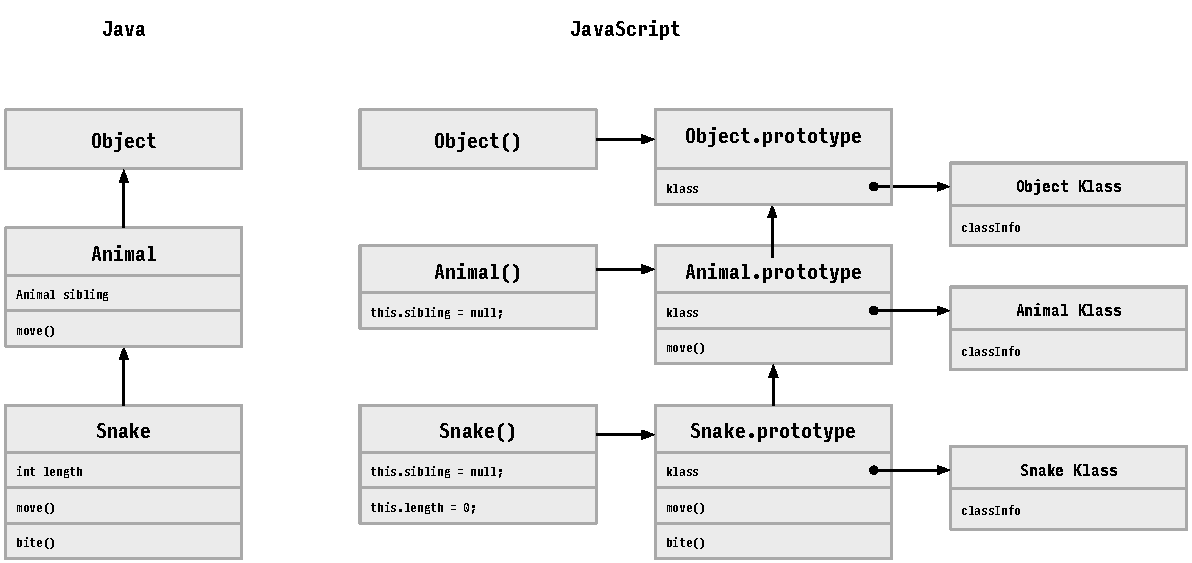
\includegraphics[height=6cm]{objects.pdf}
\caption{Object Layouts}
\label{fig:objects}
\end{center}
\end{figure*}

\subsubsection{Object}

\subsubsection{Typed Arrays}

\subsubsection{Object Arrays}

\subsection{Stack Layout}

\subsection{Interpreter}

\subsubsection{Switch Loop}

\subsubsection{Hosted Interpreter}

\subsection{Interpreter}

\subsection{Just-in-Time Compiler}

\subsubsection{Relooper}

\subsection{Threading}

A JVM that needs to run even mildly sophisticated applications must implement threads.
Java threads are typically implemented using the underlying operating system's threads.
JavaScript does not have access to the operating system's raw threads, but it does allow for concurrent programming with the use of web workers which are a similar concept to threads, but differ in key ways.
Each web worker runs in its own isolated execution context and can only share data through a copying message passing system.
Web workers also follow JavaScript's run-to-completion execution model with an event loop, which makes it impossible to lock or wait on another web worker.
With the aforementioned limitations of web workers our VM instead emulates threads entirely in the main JavaScript event loop.
This allows us to share data easily, but it still comes with a number of challenges.

\footnote{In the future web workers may be a viable option to emulate threading with the advent of shared array buffers, but at the time of creating our VM no browsers supported this option.}

\subsubsection{Asynchronous I/O, Synchronization, and Context Switching}

\subsubsection{Scheduling}

\subsection{On-Stack-Replacement}

\subsection{Garbage Collection}

\subsection{Performance Tuning}

\subsubsection{Startup Speed}

\subsubsection{Memory Usage}

\subsection{Host VM Tuning}

\subsection{Native Interface}

\subsection{Citations}

\subsection{Evaluation}

\section{Related Work}

\section{Conclusions}

\bibliographystyle{abbrv}
\bibliography{paper}  % sigproc.bib is the name of the Bibliography in this case

\end{document}
